% Theoretical background
%\clearpage%if the chapter heading starts close to bottom of the page, force a line break and remove the vertical vspace
\vspace{21.5pt}
\chapter{Theoretical background: Software And Software Testing}

This chapter explores the concept of computer software and its foundational
theory as it applies to software testing. The discussion begins with a
comprehensive overview of computer software and its historical progression.
Subsequently, the focus shifts to the crucial aspects of software testing.
The discourse culminates in an exploration of software quality from the
perspective of different quality attributes, highlighting their
significance in the development and maintenance of high-quality software systems.
%\section{Computer Software, Software Testing and Information Security}

\section{Computer Software}
Computer software, also known as programs or applications, encapsulates a set of instructions that
enable interaction with a computer or digital device to accomplish a broad array of
tasks~\cite{Software76:online}. This includes operating systems~\cite{stallings1998operating},
application software~\cite{Definiti63:online} such as
word processors or graphic design tools, and more complex systems like databases or
scientific simulations~\cite{Definiti63:online}.

Software can be classified into various categories, with one crucial distinction
being between system software, which governs the fundamental functions of a
computer or network, and application software, which executes tasks for the
user~\cite{WhatisSy89:online}\cite{Definiti63:online}.
Additionally, software can be classified as local, denoting that it operates on
the user's device, or web-based, meaning it functions on remote servers and is
accessed via the internet. A growing amount of software is crafted for handheld
devices such as smartphones and tablets, commonly referred to as mobile
applications or `apps'~\cite{yetisen2014regulation}.

The evolution of software development dates back to the 1950s and 60s when low-level assembly
languages were prevalent~\cite{lehman2002software}. However, from the 1970s onward, high-level
languages providing a greater degree of abstraction from the hardware~\cite{WhatisHa66:online}
have become the norm. For instance, the C programming language, developed at Bell Labs in the
early 1970s, has been extensively used for system programming and embedded systems~\cite{kernighan2002c}.
Python, introduced in 1991, has gained popularity in fields like web development,
data analysis, and artificial intelligence due to its emphasis on code readability and a
comprehensive standard library~\cite{van2007python}. Programming languages like
Swift~\cite{rebouccas2016empirical} and Kotlin~\cite{samuel2017programming},
introduced in 2014 and 2011 respectively, have been officially adopted by Apple and Google
for iOS~\cite{WhatIsSw25:online} and Android mobile app development~\cite{WhatIsKo37:online}.
These languages, while newer, have quickly gained traction due to their ease of use,
modern features, and support from their respective tech giants.

The emergence of these languages and many others has contributed to the rich,
diverse landscape of software development. The evolution and selection of programming
languages continue to be driven by factors such as project requirements,
efficiency, ease of use, and the ongoing growth and transformation of
technology~\cite{goosen2008brief}.

The integration of software into various aspects of modern life and business operations
has highlighted the importance of delivering high-quality, error-free software
applications~\cite{kahn2002information}. This need stems from several factors.
User expectations have heightened, necessitating software that meets functional
requirements while providing seamless and intuitive interfaces~\cite{ryker1997determinants}.
Furthermore, system reliability is crucial as software failures can result in significant
consequences such as financial losses, compromised safety, and
tarnished company reputations~\cite{pham2007system}.
Regulatory and compliance requirements also mandate specific performance and reliability standards,
especially in sectors like healthcare, finance, and aviation~\cite{mishra2022cybersecurity}. Moreover,
in today's competitive business environment, the quality of software can be a key differentiator
that affects customer loyalty and market share~\cite{rust1993customer}. Despite the importance of these
factors, many software applications still face operational failures due to insufficient adherence to
rigorous software engineering processes, such as requirements elicitation, system design,
implementation, testing, and maintenance. Therefore, robust software engineering methodologies are
crucial in mitigating potential system failures and fostering the development of reliable
software systems.

Software quality is a multi-faceted concept that encompasses various attributes determining the
extent to which a software product meets its users' needs and expectations~\cite{boehm1976quantitative}.
These attributes can be broadly categorized into functional and non-functional aspects. Functional
quality refers to the degree to which the software performs its intended tasks, encompassing factors
such as accuracy, reliability, and correctness of output~\cite{kiruthika2015software}. On the other hand,
non-functional quality pertains to the overall performance and usability of the software,
including efficiency, scalability, maintainability, usability, security, and portability~\cite{chung2012non}.
Evaluating software quality is a complex task that requires comprehensive testing and analysis
methodologies. It is integral to the entire \acrlong{sdlc}, from initial
requirements gathering to system design, implementation, and maintenance stages. High software quality
is vital as it directly impacts user satisfaction, system reliability, and the ultimate success of the
software in achieving its intended purpose. Therefore, investing in quality assurance and testing
procedures is a crucial aspect of software engineering, aimed at identifying and rectifying defects,
improving the user experience, and ensuring the delivery of robust, high-performing software
products~\cite{cavano1978framework}.

High-quality software leads to customer satisfaction, retention, and ultimately, increased profits.
\citeauthor{8748529} argue that ``a process with high-quality standards yields products with high
quality standards''.
To ensure that software is of high quality, testing is an essential step in the software development
process~\cite{8748529}.

The Figure:~\ref{fig:software_quality_perspective_1} describes different software quality perspectives
and its dependencies.

\begin{figure}[H]
    \centering
    \adjustbox{width=\textwidth}{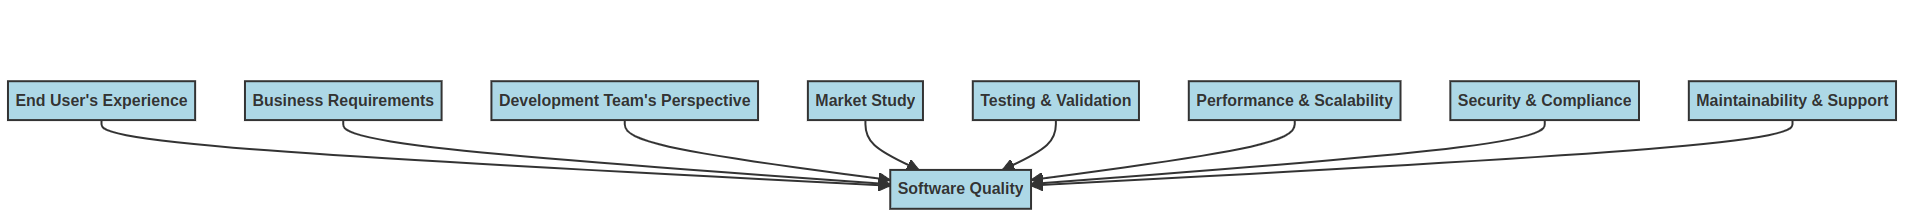
\includegraphics{software_quality_perspective_1}}
    \caption{Software Quality Perspective}~\label{fig:software_quality_perspective_1}
\end{figure}



\section{Software Testing}

According to \citeauthor{whittaker2000software}, the software testing process is often misunderstood
within the realm of software development~\cite{whittaker2000software}. It serves as a means of
evaluating and verifying a software program to determine its alignment with technical and business
requirements, as well as user expectations and overall functionality~\cite{bentley2005software}.
Additionally, as noted by \citeauthor{jamil2016software}, software testing is a risk-based activity
that aims to uncover bugs, errors, unmet requirements, and vulnerabilities. Through this process,
confidence in the behavior and requirements of the program can be gained~\cite{jamil2016software}.

Software testing is a costly endeavor, and it is impossible for any software program to be completely
devoid of bugs or errors. As depicted in Figure:~\ref{fig:software_testing_quality}, there exists a
correlation between the quality of software and the effort invested in testing. Specifically,
as the cost of testing increases, the quality of the software improves and the number of bugs
decreases in proportion to the amount of testing conducted. The criteria for the termination of
testing is contingent upon various factors, including time constraints, budget limitations, and the
scope of testing.


% \begin{figure}[ht]
% \centering
% \AltText{Testing Effort vs Quality}{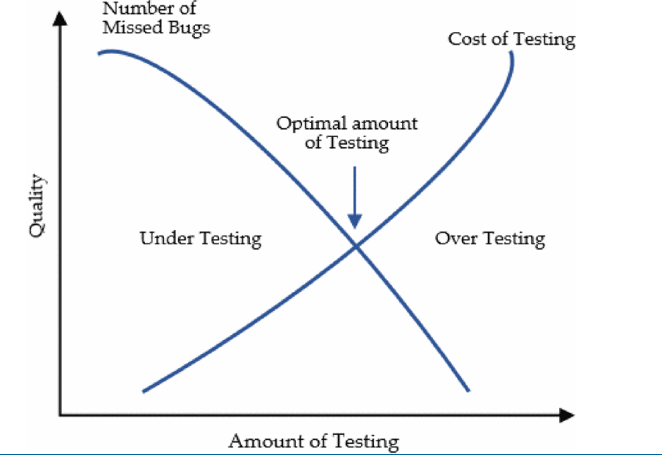
\includegraphics[width=12.1cm]{software_testing_quality}}
% \caption{Testing Effort vs Quality\cite{arumugam2019software}}\label{fig:software_testing_quality}
% \end{figure}

\begin{figure}[h]
    \adjustbox{width=\textwidth}{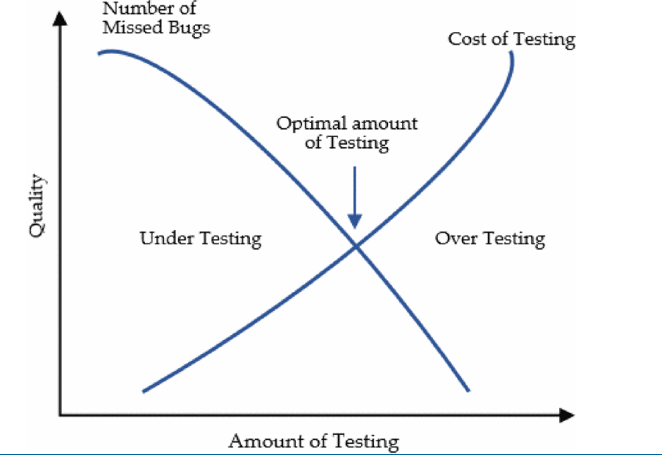
\includegraphics{software_testing_quality}}
    \caption{Testing Effort vs Quality~\cite{arumugam2019software}}~\label{fig:software_testing_quality}
\end{figure}

\subsection{Software Testing Quality Attributes}

Software testing methods and attributes play a crucial role within the \acrlong{sdlc},
contributing to the enhancement of quality processes and techniques. A key component of software
testing is static analysis techniques~\cite{zheng2006value}, which encompass inspections and reviews.
These techniques are essential attributes in ensuring the quality of the software and serve as a complement to
traditional software testing methods.

\subsubsection{Software Attributes}

Software attributes are characteristics of software testing that assist in describing the
overall quality of a software program.

The Table:~\ref{tab:software-attributes} shows the attributes of software quality~\cite{mili2015software}.

\begin{table}[H]
\caption{Software Quality Attributes}
\label{tab:software-attributes}
\begin{tabularx}{\textwidth}{lX}
\toprule
\textbf{Attribute} & \textbf{Description} \\
\midrule
Interoperability & The ability of the software to operate seamlessly in different operating systems and machines. \\
Simplicity & The ease of use, avoiding misuse, and interactions with other systems. \\
Ease of Learning & The ability of the software to adapt and improve through system interactions and output logs. \\
Customizability & The ability of the software to be configured or adjusted to meet the specific needs of a user or organization. \\
Calibrability & The ability of the software to be fine-tuned for optimal performance and accuracy. \\
Reliability & The ability of the software to perform its intended functions without failure or external influence. \\
Functionality & The features and capabilities of the software, organized in a modular manner to conceal information. \\
Portability & The ability of the software to run on different platforms and hardware configurations. \\
Reusability & The ease with which the software can be modified, adapted, and reused. \\
\bottomrule
\end{tabularx}
\end{table}

All these attributes play a crucial role in the software development process, ensuring that the
software meets desired quality standards and is user-friendly.

% \subsection{Software Testing Methods}
% Software Testing is classified into different testing methods to evaluate the correctness of the software
% in a \acrshort{sdlc}. It is an art, and is not mature and constantly evolving. Static and dynamic analysis
% are two different approaches are practiced in software testing and are important in \acrshort{sdlc}.


% \subsubsection{Static Analysis}
% Static analysis is performed early in the \acrshort{sdlc}. It helps in finding the bugs early and at this
% stage the fixing a bug is lot cheaper than fixing it in the later stage of the \acrshort{sdlc}.
% It is performed not by executing the program, but analyzing the source code.
% Static analysis tools are used to analyze the code or the program as a whole automatically.

% Below are the issues uncovered by the static analysis tools,
% \begin{itemize}
%         \item Static Bugs
%         \item Securities vulnerabilities
%         \item Unused and dead code
%         \item Syntax and semantic errors
%         \item Code complexity and Standard violations
% \end{itemize}

% \subsubsection{Dynamic Analysis}
% Dynamic analysis is opposite to the static analysis where the correctness of the software is evaluated
% by executing the software and the source code. It helps in collecting data about memory usage, performance
% and usually performed during the development, testing and production environment. For the automation,
% different dynamic tools are used.

% Dynamic tools are used to detect below issues,

% \begin{itemize}
%         \item Memory leaks and performance issues
%         \item Thread locks and garbage collection issues
%         \item Unused and dead code
%         \item Exceptions and error conditions
%         \item Code complexity and Standard violations
% \end{itemize}

%\subsection{Software Testing Types And Techniques}
% The classification of software testing into functional testing and non-functional
% testing is essential for ensuring the quality and functionality of software
% programs.

% Functional testing concentrates on verifying the software's conformity with specified requirements,
% whereas non-functional testing focuses on evaluating the software's performance, security,
% usability, and other non-functional attributes. Both forms of testing can be executed at various
% stages of the software development life cycle and can be automated through the use of specialized
% tools and frameworks.

% The Figure~\ref{fig:software_testing_types} illustrates different functional and non-functional
% testing.

% \begin{figure}[ht]
%         \centering
%         \AltText{Software Testing Types}{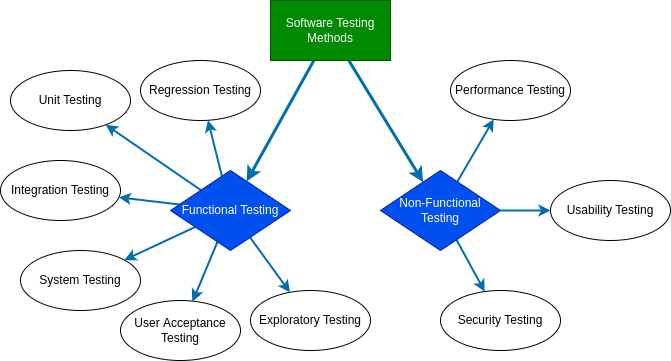
\includegraphics[width=12.1cm]{software_testing_types}}
%         \caption{Software Testing Types}\label{fig:software_testing_types}
% \end{figure}

% \subsubsection{Functional Testing}
% Functional testing is a type of testing that focuses on assessing the functionality of software
% with respect to compliance with specific requirements. This form of testing involves evaluating
% inputs, outputs, and system behaviors from the perspective of the end user to guarantee that the
% software is functioning as intended. As a result, functional testing is often referred to as
% ``specification-based testing'' as it verifies that the software adheres to the
% specified requirements\cite{Differen44:online}.

% The common types of functional testing include:

% \begin{itemize}
%         \item Unit Testing: The testing of individual components or units of a
%         program to determine their proper functioning.
%         \item Integration Testing: The testing of the integration of various
%         components or units to ensure that they interact with each other as intended.
%         \item System Testing: The testing of the entire system,
%         including units and integrated components, as a whole.
%         \item Regression Testing: The process of verifying the software after functional changes
%         have been made to other parts of the software to ensure that existing functionalities
%         still operate as expected.
%         \item Exploratory Testing: An ad-hoc and spontaneous examination of
%         the software to uncover new issues or bugs.
%         \item User-Acceptance Testing: The evaluation of the software to ensure
%         that it meets the expectations of the end-user.
% \end{itemize}


% \subsubsection{Non-Functional Testing}
% Non-functional testing encompasses a wide range of testing types that are aimed at evaluating the
% software's performance, reliability, usability, and security, among other non-functional attributes.
% These attributes are critical for determining the overall quality and suitability of the software
% for its intended purpose. Some common types of non-functional testing include load testing,
% volume testing, stress testing, security testing, compatibility testing, and
% usability testing, among others.

% These tests are designed to assess the software's ability to perform under varying conditions,
% such as high volumes of traffic, increased usage, and security attacks. The results of
% non-functional testing can provide valuable insight into the software's strengths
% and weaknesses, and can inform decisions about future development and improvement efforts.

% The common types of Non-Functional testing include,
% \begin{itemize}
%         \item The evaluation of the system's expected performance from the end user's perspective.
%         This type of testing assesses the system's throughput, response time, or a combination of
%         both, to determine its performance\cite{weyuker2000experience}.
%         \item Usability Testing: The assessment of the software's ease of use,
%         with a focus on user experience. This type of testing evaluates the software's
%         functionality, navigation, and overall usability.
%         \item Security Testing: The examination of the software to ensure that it functions as
%         intended in the presence of malicious attacks, such as hacking attempts, viruses,
%         and other security threats. This type of testing verifies the software's security features,
%         including encryption, authentication, and authorization.
% \end{itemize}

% \subsection{Software Testing Categories}
% Software testing is commonly categorized into three distinct types:
% black-box testing, white-box testing, and gray-box testing.

% These categories are defined by the level of information available during the testing process.
% In each of these categories, test cases are devised to thoroughly test the software and ensure
% its quality and functionality. The choice of testing category is determined by the extent to
% which the internal structure of the software is known and can be used to inform the
% testing process.
% \clearpage

% The Figure~\ref{fig:software_testing_categories} illustrates different software categories.

% \begin{figure}[ht]
%         \centering
%         \AltText{Software Testing Categories}{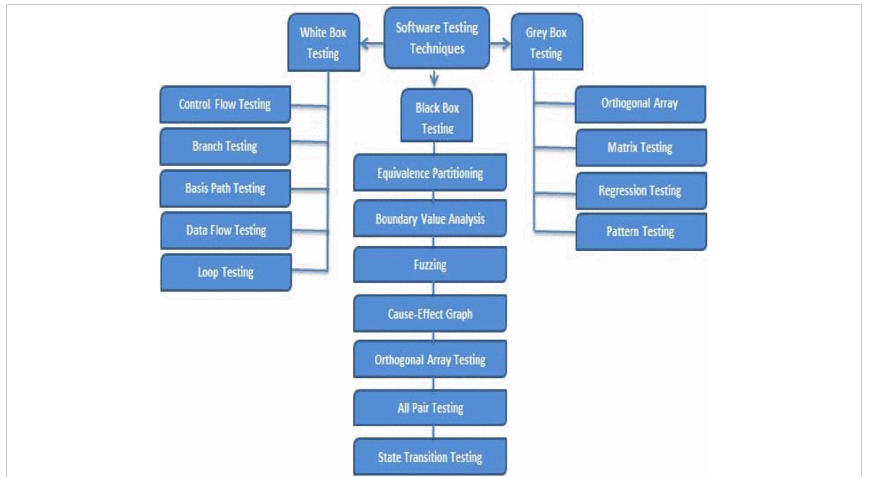
\includegraphics[width=12.1cm]{software_testing_categories}}
%         \caption{Software Testing Categories\cite{jamil2016software}\cite{jovanovic2006software}.}\label{fig:software_testing_categories}
% \end{figure}

% \subsubsection{White-box Testing}

% White-box testing, also known as ``structural testing'' or ``clear-box testing'',
% is a type of software testing that requires access to the software's source code,
% requirements, and specification documents. This type of testing is based on the software's
% internal structures and implementation details and often involves source code
% review\cite{abran2001guide}.

% White-box testing covers unit testing, branch testing, integration testing, and control flow testing.
% The process of white-box testing is typically performed by developers and requires an understanding
% of the software's internal structure. Automated test frameworks and tools, including code coverage
% tools, are often used to perform white-box testing. Fuzzing techniques can also be used to uncover
% problems. Due to early detection, bugs found during the white-box testing phase of the \acrlong{stlc}
% are generally less expensive to fix\cite{miller1981introduction}.


% \subsubsection{Black-box Testing}
% In the Black-box Testing approach, the focus is on the inputs, expected outputs, and functionalities
% of the software, without taking into consideration the internal working of the system. This type of
% testing is also known as  ``behavioral testing'' or  ``functional testing''. The testers are unaware
% of the internal workings of the software, which helps to identify any issues that may arise
% from the end-user's perspective.

% This testing technique is performed in various stages of the \acrshort{sdlc} and is widely used to
% test the functionality of the software. The test cases are designed based on the user requirements
% and functional specifications. The testers are not required to have any knowledge of the code, which
% makes it a cost-effective testing method as it does not require specialized skills or in-depth
% knowledge of the software. Automated testing tools can also be used to perform Black-box Testing,
% which can increase the efficiency and speed of the testing
% process\cite{jamil2016software}\cite{pudas2017improving}.

% Fuzzing is a commonly used technique within the Black-box Testing methodology. It involves the
% evaluation of the software's inputs, outputs, and behaviors. Black-box fuzzing is considered to
% be less complex in comparison to White-box fuzzing, and it offers faster and lighter testing but
% with limited coverage. On the other hand, White-box fuzzing is more complex, requiring more time
% and resources, but it provides a broader coverage of the software's internal structures and
% functionalities\cite{godefroid2008grammar}.

% \subsubsection{Gray-box Testing}
% The Gray-box Testing technique is a combination of the black-box and white-box testing methods,
% which is typically executed by both software developers and quality assurance teams within the
% \acrshort{sdlc}. This testing approach encompasses regression testing, pattern testing,
% and matrix testing and necessitates knowledge about both the internal architecture and end-to-end
% functionality of the software\cite{jamil2016software}.

% Reverse engineering and manipulation of the binary in black-box fuzzing can result in gray-box
% fuzzing, where the fuzzing tool inserts instructions and instrumentation into the precompiled
% black-box binary to provide the fuzzers with the necessary information. Regression testing,
% pattern testing, and matrix testing are common examples of gray-box
% testing\cite{wilson2018evaluation}.
\clearpage
% -----------------
% Academic end check

%  -----------------